%!TEX root = main.tex
\subsection{Overview}
The expert evaluation was conducted with a senior scientist at Sintef Information and Communication Technology\footnote{Sintef ICT: \url{http://www.sintef.no/home/Information-and-Communication-Technology-ICT/}}, which also has a position as adjunct associate professor at NTNU. The evaluator is an expert in the field of agile software development and knowledge management in software companies. The evaluator has published several case studies of agile teamwork in the software development industry. He also had knowledge of version-control systems, GitHub and the use of such tools in agile development teams. Apart from the expert review, the evaluator was never directly involved in our thesis.

The evaluation performed was a type of expert walk through as described in \emph{Interaction Design - Beyond Human Computer Interaction}\cite{rogers2011interaction}. The evaluation we performed differs in that we also evaluate how the application can support agile software development teams and reflection through revisiting experiences. \\ 
The evaluation started with us presenting the main features of the application and then continued with a walk through of the application in its production state. The walk through consisted of performing the typical tasks in our scenarios. After the walk through we had an open discussion around the most common challenges agile development teams meets.  The evaluator also commented on possible shortcomings or limitations, and also any advantages the evaluator had identified in our application. We asked the evaluator to present his ideas on how our application could improve reflection in agile software development teams. We wanted an objective evaluation so we did not initially present any of our own thoughts regarding the application and its goals. \\

The evaluator suggested several possible limitations in the application, and also commented on how our application met some of the problems that often arise in development teams and how he could see our application potentially help limit these problems. We particularly went through the reflection workshop questions, to get feedback on the feasability of these and triggering reflection in a retrospective session [See Figure \ref{workshopmandatoryexpertreview}]. 

\begin{figure}[H]
    \centering
        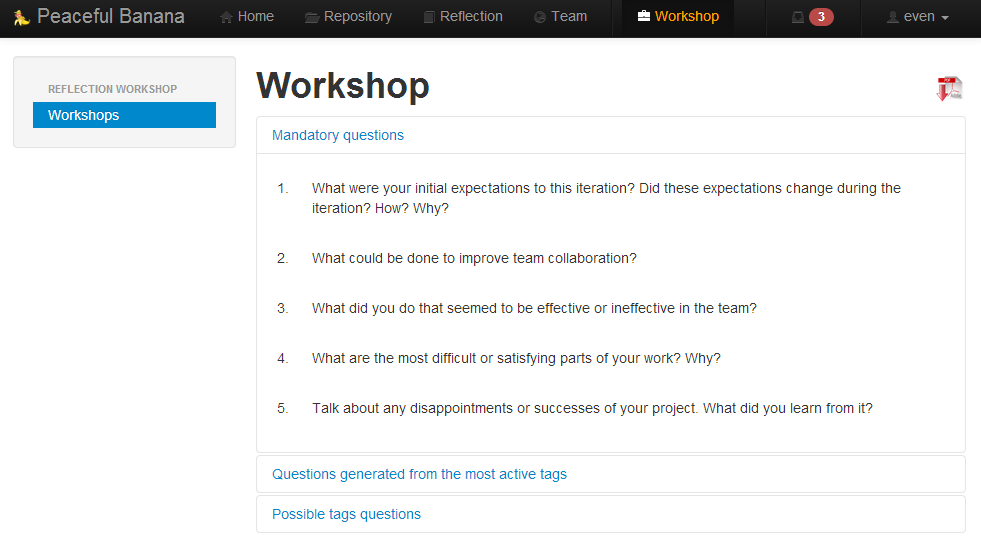
\includegraphics[width=\textwidth]{workshopmandatory}
    \caption{Example of retrospective session questions to trigger reflection.}
    \label{workshopmandatoryexpertreview}
\end{figure}

In addition to advantages and limitations of our application, the evaluator had some input towards related work he had seen, and how we could conduct the final evaluation in the best way. This included possible questions that might be relevant to ask the participants, how to get the best possible output from these and also some theory on how to analyse the results we got. \\
The feedback we got from the expert showed that the application had features that met many of the problems he had encountered through his studies of agile teams, and specifically how to trigger and enhance reflection. The evaluator also had some valuable feedback on possible shortcomings in the application, which can be typical challenges developers face in a day to day working environment. 

\subsection{Overall Feedback}
The evaluation with the Sintef expert left us with the impression that the evaluator was satisfied with the general functionality of the application, in terms of agile teams and reflection in these teams. 
At the point of evaluation, the application had been deployed to production state, and so most of the functionality was in place. The evaluator stated that the choices we had made on the data collection and representation of these was satisfying, as it allowed and encouraged users to reflect on their experiences, while not being too intrusive on the daily work routine. Both in aspects of individual and collaborative reflection the application and its functionality was satisfactory. \\

As for integration of the tool, the evaluator saw a limitation in that it was generally hard to get new tools into the daily routine of developers\cite{rogers2010diffusion}, and referred to the Technology Adoption Curve by Rogers[Figure \ref{rogerscurve}. The way we encourage users to use \#\emph{hashtags} to tag important elements in the commit message, might take some time to work in. The evaluator expressed that he was happy with the design choices made and that we chose a web-application as a platform. This way the application is available for all individuals in the team, on a wide variety of devices. This availability is important in order to further lower the threshold of usage. Apart from general feedback and app-specific feedback we also got some feedback regarding the final evaluation. Specifically what questions to ask, comparing their previous retrospective routines with a retrospective using our application beforehand. Also feedback on how to properly analyse the results we would get was valuable. The evaluator had identified possible reasons for why a certain outcome could occur through his studies. The evaluator was also pleased with the notion of allowing teams to see what notes are shared , which allowed for identification of \emph{sharing patterns} among the users. This is something that could help encourage a \emph{"discussion about reflection in the retrospective sessions"}. Another point was that individual users tend to use the same tools in different ways, so specifying what and how the application could be used before users started using the tool was important.  
\subsection{App-specific feedback}
Here we will present the challenges the evaluator presented in the aspect of teamwork and reflection in agile software development teams. The challenges identified in Table \ref{experttable} was used to create a discussion around the PeacefulBanana application and how it can solve these problems. 
\begin{figure}[H]
    \centering
        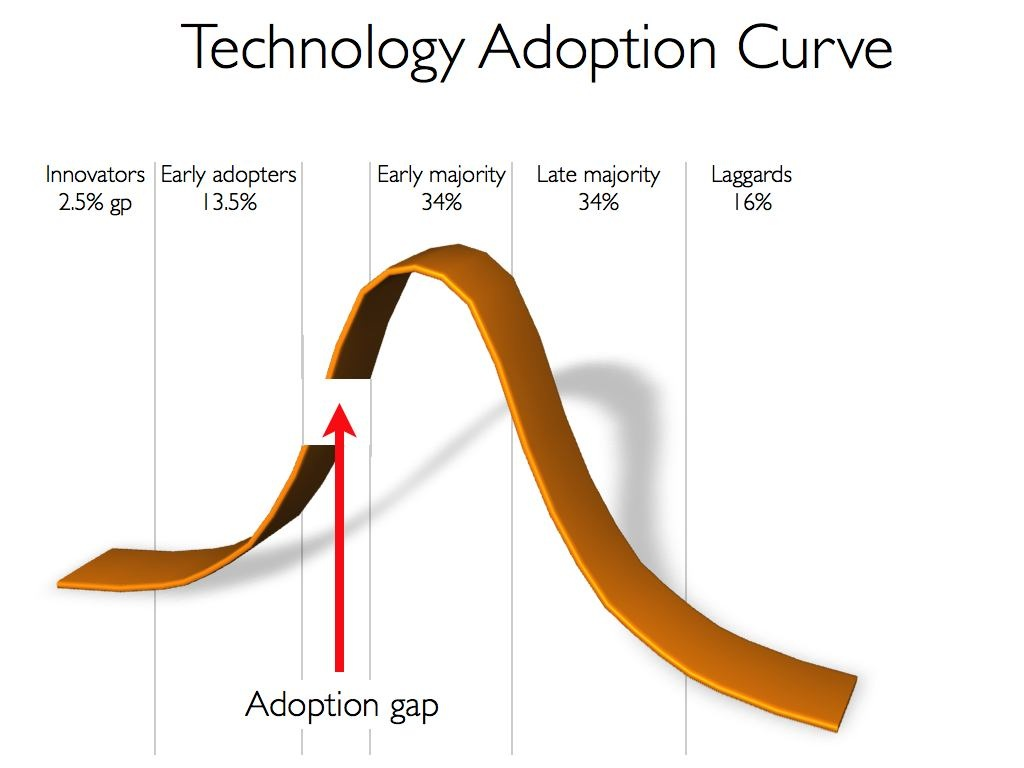
\includegraphics[width=\textwidth]{rogerscurve}
    \caption{Roger's Innovation Adoption Curve}
    \label{rogerscurve}
\end{figure}

\newpage

\begin{table}[H]
    \begin{tabularx}{\textwidth}{|l|l|X|}
    \hline
    ID & Name                & Description                                                                                                                                                                                                                                                                                                                                                    \\ \hline
    1  & Non-intrusive       & The threshold of integrating new tools into the routines of software developers is hard. The evaluator specifically referred to the \emph{Technology Adoption Curve} presented by Rogers\cite{rogers2010diffusion}, which refers to the chasm between innovators or early adopters and the early majority. This curve can be seen in Figure \ref{rogerscurve}. \\ \hline
    2  & Uniqueness          & The application should meet a demand which hasn't already been met. Also the application should provide something that a normal retrospective does not.                                                                                                                                                                                                        \\ \hline
    3  & Agile integration   & How can the application be integrated into an agile environment, helping the team to be agile and not removing the agility from the team.                                                                                                                                                                                                                      \\ \hline
    4  & Dynamic Memories    & Memories are dynamic and change over time, so there can be a lack of memorizing all important situations in a retrospective.                                                                                                                                                                                                                                   \\ \hline
    5  & Priorities          & Often agile teams develop what the developers are motivated for, and not what the customer prioritizes highest. These wrong-placed priorities can be hard to pick up.                                                                                                                                                                                          \\ \hline
    6  & Competence-overlap  & Agile teams are most efficient and deliver the highest quality work when at least two people have the same competence, so that one can ask for help and code can be reviewed by a peer. When a developer is left alone on a piece of work, integrating these parts with the rest of the project can be an issue                                                 \\ \hline
    7  & Re-work:            & Re-doing the same piece of work is also a challenge development teams can meet. When developers constantly revisits work that already has been accepted, to make unnecessary changes, the progress of the project is slowed down. Detection of this can allow for a discussion and allowing the team to progress.                                              \\ \hline
    8  & Level of expertise: & Developers often have different levels of expertise, and different areas of expertise. Even though a developer have a high amount of impact on the code-lines committed to a project, this does not mean the others don't do important work.                                                                                                                    \\ \hline
    \end{tabularx}
    \caption {Expert review feedback}
    \label{experttable}
\end{table}

\clearpage

\begin{itemize}
    \item 1. Non-intrusive:
\end{itemize}
The evaluator was satisfied with the design choice we made. By keeping the amount of time users are \textbf{required} to put into the application to a minimum, the threshold of usage is kept as low as possible at the same time. As mentioned, the Roger's adoption curve state that integrating a new tool into a daily routine is hard already, so it's important the users don't feel the application is a necessity but a helpful tool. The evaluator specifically mentioned that the daily reflection note was a good choice, since it only takes roughly 5 minutes and serves a purpose for the users. If the users then should wish to dive further into the functionality, it is easy accessible. 

\begin{itemize}
    \item 2. Uniqueness: 
\end{itemize}
The feedback here was that the evaluator had not encountered a similar tool during his research, and he felt the application met a need in the industry. As for the retrospective aspect, the feedback was that the application had features for identifying issues and situations that in a normal retrospective could be lost.  

\begin{itemize}
    \item 3. Agile integration: 
\end{itemize}
The evaluator expressed a certain concern that too much data collection could lead to an overhead in the amount of data that needed to be analysed during the retrospective. Emphasis here was that the application shouldn't come in the way of the team being agile. 

\begin{itemize}
    \item 4. Dynamic Memories:
\end{itemize}
 The evaluator stated that by implementing the daily reflection note feature, we allowed for the most important experiences of the day being collected and stored for later use. This means that although not all data or experiences are collected, the application encourages users to reflect on fresh memories and can revisit these later during the retrospectives, hopefully omitting the risk of forgetting certain situations. 

\begin{itemize}
    \item 5. Priorities: 
\end{itemize}
The evaluator stated that this is a common problem in development teams, and thus allowing for identification of such mis-priorities are important. The feedback was that the application features for seeing how far the team has come in the particular milestones, and going into the separate issues to see when it has been worked on and by who, partially had met this challenge. The evaluator still expressed that this could be even more emphasized, and be made more easily accessible. 

\begin{itemize}
    \item 6. Competence-overlap:  
\end{itemize}
Through the different tag clouds featured in the application, a missing overlap in competence can be identified. The evaluator stated that comparing the team tag cloud with the personal tag cloud was a satisfactory way of identifying whether an individual has been working a lot alone. Further feedback was that some sort of comparing tag clouds between individuals would further help towards this challenge, but this could in turn lead to unwanted focus on individuals performance.

\begin{itemize}
    \item 7. Re-work: 
\end{itemize}
 Also here the feedback was that inspection of issues allows for seeing when and how often a problem has been fixed and then re-opened again. Also by comparing tag clouds from different periods allow for identification of much re-work. Even though the functionality was there, the evaluator wanted to make these comparisons more easily accessible in the application.

\begin{itemize}
    \item 8. Level of expertise:   
\end{itemize}
The feedback here was: Since the application focuses on project commits and comparing the users activity based on the work committed to GitHub, the application could give the wrong impression of how much work individuals in the team have done. Because of this the evaluator emphasized that we kept this fresh in mind, when describing what the tool is, what it does, what it measures and most importantly what it doesn't measure. This is important so that no users feel their work is diminished in importance by using the application.

\subsection{Features}
During our discussion with the evaluator we identified some features that were missing which could be fitting to implement in the application:
\begin{itemize}
	\item \emph{What is new?} functionality:
\end{itemize}
Show parts of the source-code in the PeacefulBanana application, creating a sort of \emph{What has happened since your last visit} functionality to the users and teams. The evaluator proposed that having such functionality might increase the user's motivation to use the application, and further trigger reflection for the daily reflection notes. 
\begin{itemize}
	\item Burn down-Chart:
\end{itemize}
The evaluator proposed including a burn down-chart based on the issues already existing on GitHub and in the PeacefulBanana application. A burn down chart is a graphical representation of work left to do versus time. The tasks or issues remaining(the backlog) is often on the vertical axis, with time along the horizontal axis.\\
A burn down chart is useful for estimating or predicting when all of the work or issues will be completed. In agile software development teams, it is a common tool to measure progress over time. The application supports some progress viewing in each milestone by presenting users with a progress bar, although the evaluator stated that a burn down-chart feature would be an addition teams would use and such increase the motivation for using the application as a whole. An example of such a burn down-chart can be seen in Figure \ref{burndownchart}. 
These features were noted as feature work, as implementing these could prove valuable for future users. 

\begin{figure}[H]
    \centering
        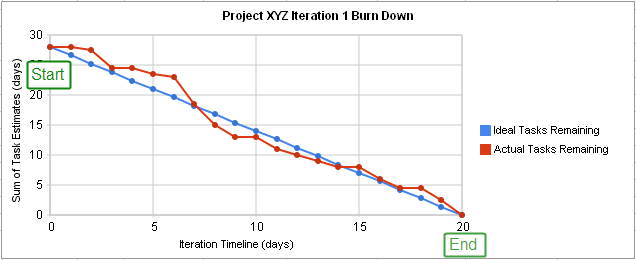
\includegraphics[width=\textwidth]{burndownchart}
    \caption{Example of a project burn down-chart}
    \label{burndownchart}
\end{figure}
\clearpage
